\documentclass{article}
\usepackage[spanish]{babel}   
\usepackage[numbers,sort&compress]{natbib}
\usepackage{float}
\usepackage{listings}
\usepackage{graphicx} 	% Nos permite importar imagenes 
\usepackage{subcaption}
\usepackage[left=3cm,right=3cm,top=3cm,bottom=3cm]{geometry}

\title{Reporte Tarea 1}
\author{Victor Alejandro Oviedo Martínez}



\begin{document}
\maketitle
\hrule
\section{Introduccón}\label{intro}

Para esta primera tarea se ha estudiado el movimiento Browniano, el cual nos habla acerca de la representación de una partícula la cual tiene la capacidad de realizar movimiento al azar con dirección y magnitud discretizados, tomando en cuenta que su posición inicial será el origen\citep{DRA.P1}. Una vez estudiado las capacidades del movimiento Browniano se ha podido ver simulaciones ejemplo con el fin de entender la tarea a realizar.

\section{Desarrollo}

Para esta primera tarea se ha planteado el siguiente problema:
Examina de manera sistemática los efectos de la dimension en el tiempo de regreso al origen del movimiento Browniano para dimensiones 1 a 8 en incrementos lineales de uno, variando el numero de pasos de la caminata como potencias de dos con exponentes de 5 a 10 en incrementos lineales de uno, con 50 repeticiones del experimento para cada combinación. Grafica los resultados en unas sola figura con diagrama de caja de bigote o violin, colocando y coloreando los resultados de una distancia y otra de tal manera que es fácil concluir si la distancia utilizada tiene algún efecto en el comportamiento, o en su defecto, incluir un cuadro indicando el mínimo, promedio máximo del tiempo de regreso por cada dimension junto con el porcentaje de caminatas que nunca regresaron\citep{DRA.P1}.\\



El programa empieza importando librerías importantes, como la generación de números pseudo-aleatorios, la librería para graficar, y la librería para la función  \texttt{Inf}.   Después se inicializan variables para los \texttt{contadorx(x,y), contadory(y)}, luego tendremos la definición de las funciones las cuales empiezan con el \texttt{contadorx(x,y), contadory(y)} siguiendo con la función \texttt{paso(pos,dim)} y \texttt{experimento (largo, dim, tiempo, t, x, y)}.

\begin{lstlisting}[language=Python]
from random import random, randint
import matplotlib.pyplot as plt
import math

x = 4
y = 4
t = 0
tiempo = 0
\end{lstlisting}



\texttt{contadorx(x,y), contadory(y)}.- Estas dos funciones funcionan en conjunto, ya que el propósito del contador X es contar del numero 5 hasta el 10, sin embargo, esta función no tiene la posibilidad de auto guardarse el valor para el reinicio, por lo tanto, se utiliza Y para recordar su posición.

\begin{lstlisting}[language=Python]
def contadory(y):
    if y < 10:
        y = y + 1
    else:
        y = 5
    return y

def contadorx(x,y):
    x = y
    if x < 10:
        x = x + 1
    else:
        x = 5
    x = 2**x
    return x
\end{lstlisting}

\texttt{paso(pos, dim)}.- Esta función se encarga de elegir una dimensión, una vez elegida una dimensión se procede ha elegir dirección para moverse. Una vez realizado el movimiento, la función regresa el vector generado.


\begin{lstlisting}
def paso(pos, dim):
    d = randint(0, dim - 1)     	# Elegimos dimension
    pos[d] += -x if random() < 0.5 else x  # Elegimos direccion y nos movemos
    return pos        			# Actualizamos el paso realizado
\end{lstlisting}

\texttt{experimento (largo, dim, tiempo, t, x, y)}.- Genera siempre un vector de posición en el origen, para después repetir la secuencia conjunta de \texttt{contador(x,y)},\texttt{ contador(y)} y \texttt{paso(pos,dim)}, esto con el fin de contar el tiempo que tarda la partícula en regresar al origen, de no regresar al origen en el tiempo máximo asignado,  se le asignará el valor infinito.

\begin{lstlisting}[language=Python]
def experimento(largo, dim,tiempo, t, x, y):
    pos = [0] * dim     	#Generando vector de posicon en el origen
    for o in range(pasos):     # Cantidad de pasos a realizar
        if t == 0:
            x = contadorx(x,y)       # Contador de 5 a 10
            y = contadory(y)        # Memoria del contador x
            pos = paso(pos, dim)     # Actualizamos pos
            if all([p == 0 for p in pos]):
                t = t + 1
            else:
                tiempo = tiempo + 1
                if tiempo == pasos:
                    tiempo = math.inf
    return tiempo
\end{lstlisting}

Después de definir algunas funciones se realiza la inicialización de algunas variables como; rep, largo, total, pasos, y Datos. Estas se inicializan en este punto para tenerlas con mayor presencia, ya que tienen mayor importancia para este programa. Se podría decir que el programa inicia con el ciclo “for i in rep:”, en donde este tiene la función de repetir el experimento para las 8 dimensiones necesarias, y que a su vez repetirá las funciones \texttt{contadorx(x,y)}, \texttt{contadory (y)}, y \texttt{paso(pos, dim)}, con el fin de simular todos los experimentos. Por último, todos los vectores de los diferentes experimentos se agrupan en una sola variable para poder ser graficados. \\

Para este reporte se tuvo la  revisión el día miércoles 16 de Septiembre del 2020\citep{DRA.CONV}, ese día se tuvo la oportunidad de corregir errores, sin embargo se  decidió dejar los errores de código en letra cursiva con el fin de reportar los errores obtenidos.\\

\textit{Ahora se hará mención ha los detalles que se tuvieron con este programa, y no se encontraron solución. Revisando el programa que la maestra dejo como ejemplo, se tiene que, para graficar todos los valores generados por el programa, estos valores son agregados a una sola variable, en la cual cada ves que se generan los datos para una sola dimensión se agregan, y dado que este proceso se repetirá hasta completar el total de dimensiones, es solo cuestión de variar el vector en el cual se guardaran nuestros datos para al final tener todos los valores en una sola variable y con esto poder graficar todo el contenido.  Este procedimiento se intento exactamente como la maestra lo realiza en su código, sin embargo, al momento de correr el programa nos genera un error en el cual nos dice que en la línea 91 la variable en la que queremos agregar los datos no tiene el rango necesario. Siendo que sí son del mismo tamaño. Se ha dejado el código utilizado comentado sobre el código de la tarea para que se pueda ver a lo que hago referencia. Sin embargo, he intentado con un rango más amplio y sea tenido el siguiente resultado.}\\

\begin{figure}[H]
\begin{center}
	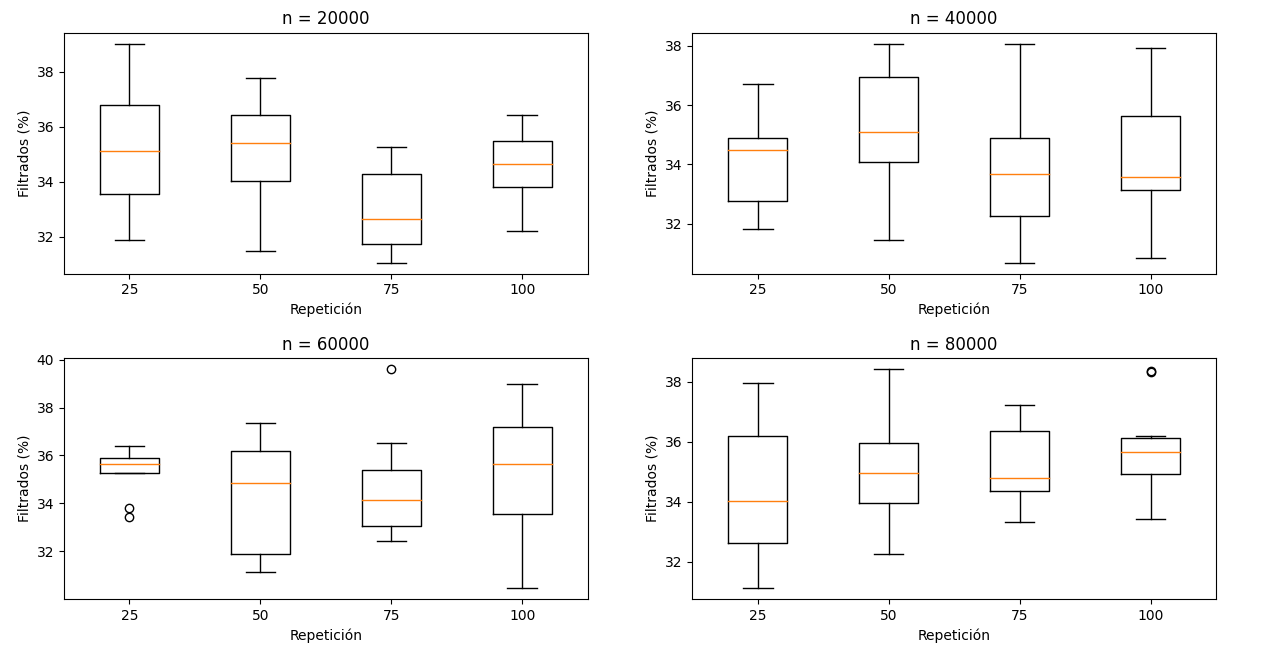
\includegraphics[height=3in]{/Users/victor/Desktop/Figure_2.png}
	\caption{Grafica con el error de rango}
	\label{fig:tarea.1}
\end{center}
\end{figure}


\textit{Cómo se puede observar en la Figura \ref{fig:tarea.1}, se pudo graficar los valores, sin embargó queda sin valores la dimensión 1. Por lo tanto, se guarda por así decirlo de forma manual los valores en la variable. Para después esta ser graficada. Por ultimo, se logro graficar todos los valores de forma manual, pero correcta, sin embargó al código se le generan errores creo yo por el uso del valor \texttt{Inf}, ya que en el proceso de conteo para el tiempo de regreso se a dejado un limite de pasos para este fin, de sobrepasarse este limite el programa esta programado para guardar el valor \texttt{Inf} como resultado a ese experimento, por lo que imagino que al momento generarse la grafica, esta utiliza todos los valores guardados en el vector de datos y al tener valores infinitos se genera un error para el calculo de la misma.}\\

Para el error de rango de la Figura \ref{fig:tarea.1}, se obtuvo la ayuda de la Dra. \citet{DRA.CONV}, la cual nos hizo reestructurar la forma en la cual se guardaban los datos obtenidos. A continuación se podrá observar el código con el cual se generaba el error.

\begin{lstlisting}[language=Python]
rep = [d for d in range(1,9)]     
Datos = [ [] for d in rep]

for i in rep:
    regresos = [0]*total        
    dim = i
    for replica in range(total):
        regresos [replica] += experimento(largo, dim, tiempo, t, x, y)
    Datos [dim] = regresos
\end{lstlisting}

En este código se generaban dos variables, en donde la primera con el nombre \texttt{rep} sirve para generar un rango con el total de dimensiones a simular, la segunda seria la variable en la cual serian guardados los resultados de la simulación. Continuando con el código, se tenia un ciclo \texttt{for} con el fin de generar las replicas necesarias del experimento. Para esto seria necesario crear una variable con el nombre \texttt{regresos}, la cual guardaría los valores de un experimento por vez, para después guardar los valores en la variable \texttt{Datos} en la posición de la dimensión correspondiente. De esta forma se guardarían todos los datos en una sola variable.  Una vez analizado los cambios que a sugerido la Dra.\citet{DRA.CONV}, sé ha podido encontrar el error en este código. El error que se ha tenido en este código, ha sido producido por la asignación  de rangos en las variables, ya que estas están desfasadas, y por lo tanto al intentar guardar los primeros valores de la primer dimensión se tiene que no existe espacio asignado en la variable, por lo tanto, no es posible realizar el programa completo, sin embargo,  la lógica de asignación de posición para la variable \texttt{Datos} es correcta para \texttt{N} dimensiones.\\

A continuación, se podrá observar el código sugerido  por la Dra. \citet{DRA.CONV}:\\

\begin{lstlisting}[language=Python]
Datos = []

for i in rep:
    regresos = []       
    for replica in range(total):
        regresos.append(experimento(largo, dim, tiempo, t, x, y))
    Datos.append(regresos)
\end{lstlisting}

Como se pudo observar el código es muy similar, sin embargo  este es mas sencillo, esto fue posible gracias a la ayuda de la función \texttt{append()} la cual agrega nuevos elementos al final de la variable, por lo que ya no seria  necesario llevar el control de la dimensión dado que al siempre empezar desde la primera dimension la función solo se encargaría de agregar los nuevos valores al final del arreglo. Gracias a este ajuste, el programa entrega los valores de forma correcta.\\

Ahora una vez conseguido los datos de cada dimensiones se realizó un filtro, este con el fin de eliminar los datos \texttt{Inf} ya que al momento de realizar la grafica el programa tiene errores dado que no se puede realizar cálculos con este tipo de valores, otra forma de representar estos valores seria por medio de un cero, sin embargo este valor afectaría la grafica al promediar conjuntos con este valor. Por lo tanto, el filtro a realizar tendría que separar los valores nulos de los que nos reflejan un resultado. Este filtro se ejecutara después del desarrollo de todos los valores.\\

A continuación, se presenta el código del filtro:

 \begin{lstlisting}[language=Python]
#-------------------------FILTRO-------------------------
print("")
print(" Regreso al origen")
for dimencion in range(max(rep)):
    for filtro in range(total):
        cont = cont + 1
        if Datos[dimencion][filtro] == 1:
            INF = INF + 1
            if cont == total:
                DatosINF.append(DatosFIL)
                DatosFIL = []
                cont = 0
                PORINF = porinf(INF, total)
                print("Dimencion", dimencion + 1,":" ,PORINF, "")
                PORINF = 0
                INF = 0

        elif Datos[dimencion][filtro] != 1:
            DatosFIL.append(Datos[dimencion][filtro])
            if cont == total:
                DatosINF.append(DatosFIL)
                DatosFIL = []
                cont = 0
                PORINF = porinf(INF, total)
                print("Dimencion", dimencion + 1,":" ,PORINF, "")
                PORINF = 0
                INF = 0
print("")
\end{lstlisting}

Para el análisis progresivo de este filtro se ha hecho uso de dos ciclos \texttt{for} concatenados, estos con el fin de recorrer cada uno de los elementos ya creados y guardados en la variable \texttt{Datos}. Cada uno de estos datos serán filtrados con la ayuda de condicionales \texttt{if} los cuales separaran datos importantes, de los datos que nunca regresaron al origen, tomando en cuenta que se llevara un conteo de estos para su posterior análisis. Una vez filtrados los datos  se guardan en la variable \texttt{DatosINF}. Por ultimo, se grafican los valores ya filtrados.\\


Dado que al momento de realizar esta practica no se tenia conocimiento alguno del programa Python, se a utilizado la introducción para uso básico de python de la Dra. \citet{DRA.COM.USOBASICO}. Para el desarrollo de este archivo se utilizo como referencia el manual \citep{manual.python}.



\section{Conclusión}



Como concusión a los resultados de la Figura \ref{fig:exp50}, y a la experiencia dejada por el desarrollo de esta tarea, se tiene que, para todas las dimensiones simuladas en este programa el tiempo de regreso más frecuente se tiene en los primeros movimientos, ya que es más probable avanzar un paso, y luego retrocederlo en la misma dimensión, que avanzar en diferentes y luego esperar que se genere el regreso en las mismas dimensiones. Aunado a la explicación anterior, se puede observar como mientras menos dimensiones se tengan más aumenta el tiempo de regreso al origen. Con esto se reafirma nuestra suposición. Dado que la cantidad de repeticiones del experimento es baja, se decidió realizar una mayor cantidad con el fin de obtener mayor precisión en la visualización de los valores, como resultado de esta acción se tienen los resultados de la Figura \ref{fig:exp5000} y el Cuadro \ref{fig:cuadro1}. Cómo se puede observar en el Cuadro \ref{fig:cuadro1}, se tiene los valores del porcentaje de regreso para 5000 y 50 repeticiones, de los cuales podemos mencionar la similitud entre los valores de los porcentajes. Sin embargo, dada la cantidad de repeticiones tenemos que los datos con 5000 repeticiones son 1000 más exactos que el experimento con 50, esto se pude ver a simple vista comparando las Figuras \ref{fig:exp5000} y \ref{fig:exp50}, dado que en la Figura \ref{fig:exp5000} se observa una grafica suavizada en comparación a la Figura \ref{fig:exp50}, en la cual se observa una grafica menos exacta. De esta forma se concluye de forma exitosa la tarea 1.   \\



\begin{table}
\centering
\caption{Porcentajes de regreso al origen .}
\label{fig:cuadro1}
\begin{tabular}{|cc|cc|}
\hline
5000 experimentos && 50 experimentos &  \\
\hline
Dimensión & Porcentaje & Dimensión & Porcentaje\\
\hline
1& 90.39&1& 88\\
2&55.74&2&56\\
3&31.28&3&38\\
4&19.16&4&26\\
5&14&5&18\\
6&10.92&6&8\\
7&9.34&7&4\\
8&7.46&8&8\\
\hline
\end{tabular}
\end{table}




\begin{figure}
 	\centering
 	\caption{Tiempo de regreso al origen y porcentaje con 5000 experimentos.} 
	\label{fig:exp5000}
 	\begin{subfigure}[H]{0.45\linewidth}
 		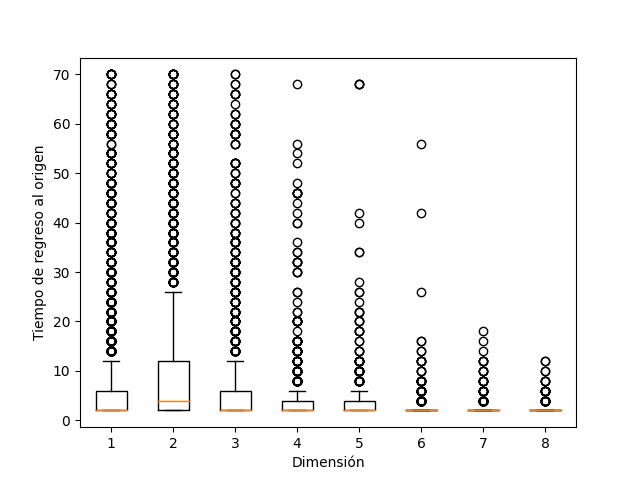
\includegraphics[width=\linewidth]{/Users/victor/Desktop/Figure_4.png}
 	\end{subfigure}
 	\begin{subfigure}[H]{0.45\linewidth}
 		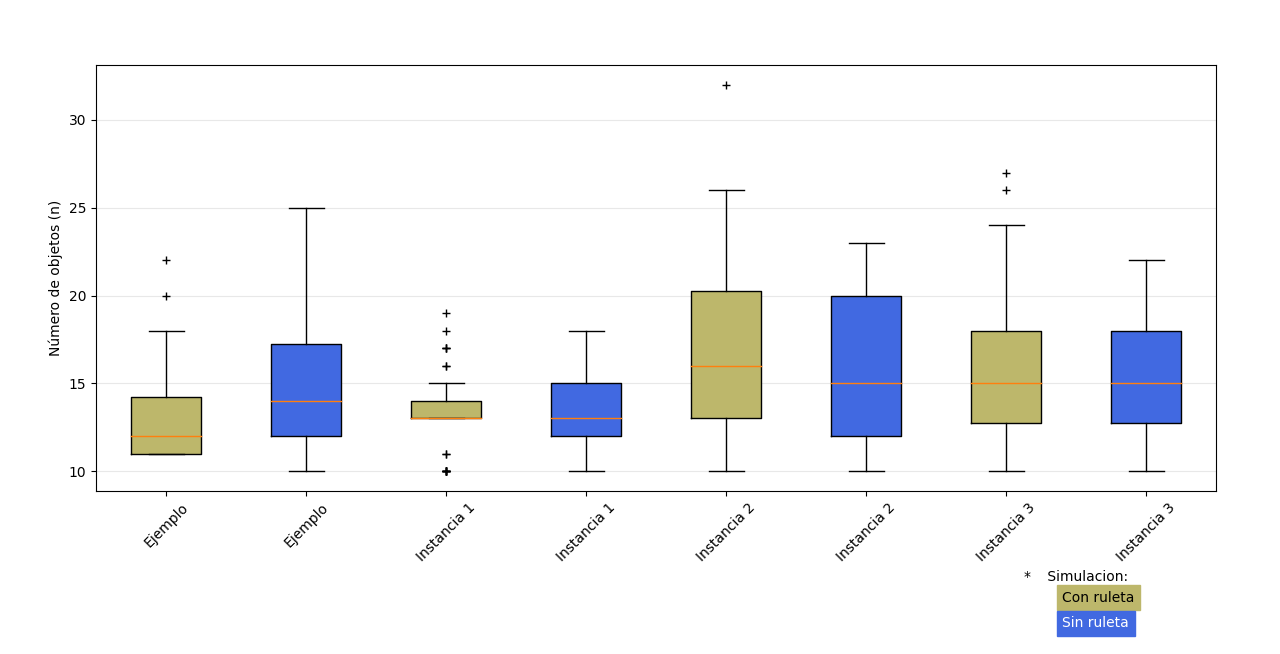
\includegraphics[width=\linewidth]{/Users/victor/Desktop/Figure_5.png}
 	\end{subfigure}
	\caption{Tiempo de regreso al origen y porcentaje con 50 experimentos.} 
	\label{fig:exp50}
 	\begin{subfigure}[H]{0.45\linewidth}
 		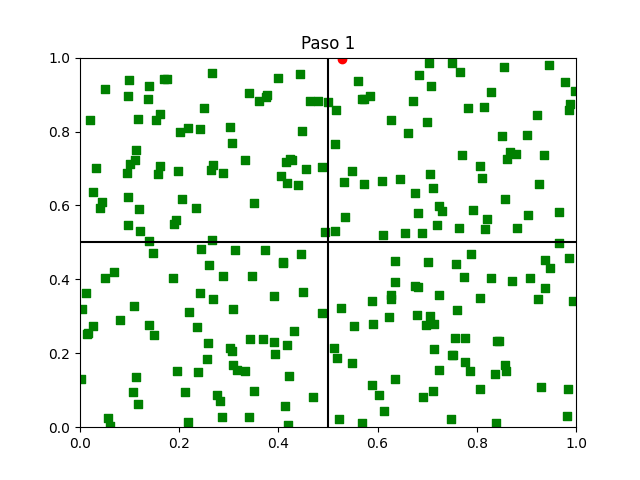
\includegraphics[width=\linewidth]{/Users/victor/Desktop/Figure_3.png}
 	\end{subfigure}
	\begin{subfigure}[H]{0.45\linewidth}
 		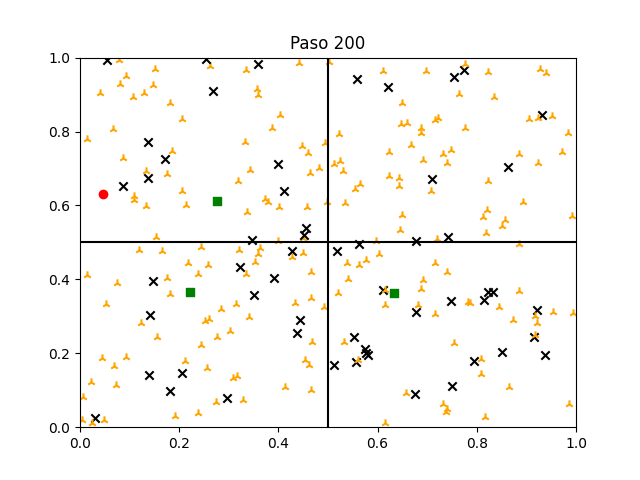
\includegraphics[width=\linewidth]{/Users/victor/Desktop/Figure_6.png}
 	\end{subfigure}
 \end{figure}

\bibliography{ref.Tarea1.bib}
\bibliographystyle{plainnat}

\end{document}
